\section{Discussion \& Conclusion}
\label{sec:conclusion}

In this work, we study the scaling properties of different techniques used in RL for LLMs in pursuit of a predictable scalable recipe. With this mission, we derive a method for fitting predictive scaling fits for accuracy on the validation set that allows us to quantify the asymptotic performance and compute efficiency of an RL method. Using this methodology, our primary contribution is to conduct a careful series of ablations of several algorithmic options that go into the RL recipe.
For each ablation, we choose the option with higher asymptotic performance when possible and improved efficiency otherwise. 
Combining these choices yields the \scalerl\ recipe which scales better than all existing recipes in our experiments.


\begin{figure}[t]
    \centering
    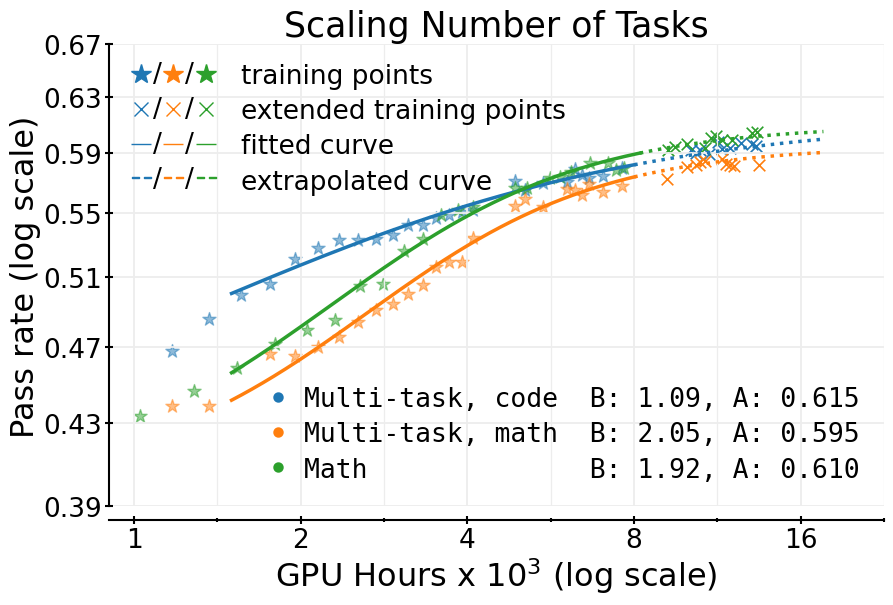
\includegraphics[width=0.6\textwidth]{paper_figs/large_scale_tasks.png}
    \caption{\textbf{\scalerl\ scales predictably on math and code}. We report both the code and math validation set performance on the joint math+code RL run; along with the math only \scalerl\ run as a reference. These results demonstrate that our sigmoidal compute–performance relationship holds across task mixtures, and that \scalerl’s scalability generalizes beyond a single domain training.}
    % For RL training, we use the Polaris-53k~\citep{polaris2025} and  DeepCoder~\citep{deepcoder2025} datasets for math and code, respectively.}
    \label{fig:scaling_math_code}
\end{figure}


A few observations are in order:
\begin{itemize}
    \item \textbf{Compute scaling extrapolation}. An important insight of our scaling methodology is that we can use smaller-scale ablations in a systematic way to predict performance at larger scales. This allows us to create our final scalable recipe.
    \item \textbf{Most important decisions}. The off-policy algorithm, loss function, and model precision are the most important decisions from our ablations. Each of the other decisions does not have a large individual effect, but as we see from the leave-one-out experiments, they still do have some cumulative impact (in terms of efficiency) when all combined. 
    \item \textbf{Asymptotic performance vs. efficiency}. For many of our ablations, we found the better option to improve both efficiency and asymptotic performance, but this is not always the case (e.g. for FP32, \Cref{fig:fp32}). When doing the ``forward'' ablations starting from the baseline method, we opt for asymptotic performance first and foremost. Interestingly, when doing the ``backward'' leave-one-out ablations from the \scalerl\ recipe, we find very little impact on asymptotic performance from each decision, but each component of the algorithm seems to help efficiency. This shows that the cumulative effect of the changes is quite robust.
    \item \textbf{Generalization}. While we report transfer to downstream evaluations, our primary focus is on studying predictive scaling, which is characterized through in-distribution performance curves on a held-out dataset from training prompts ~\citep{misfitting,scalingdataconstrained}.    
    This still leaves the question of how well the LLM would generalize from the training distribution to held out test sets. %which could be tricky as we run many epochs over the RL training prompts. 
    While a full characterization of generalization is beyond the scope of our work, we do observe correlation between in-distribution validation and downstream generalization performance. However, there are some algorithmic choices that seem to help generalization more, that we want to note here including: larger batch size (\Cref{appendix:downstream_perf}), reducing truncations (\Cref{appendix:truncations}), longer generation lengths (\Cref{sec:diff_axes}, \Cref{fig:large_scale_gen_len}), and larger model scale (\Cref{sec:diff_axes}, \Cref{fig_100k_main}).

\item \textbf{Multi-task RL}. While our  experiments focus mainly on the math domain, we also evaluate \scalerl\ under multi-task RL training. As shown in \Cref{fig:scaling_math_code}, joint training on math and code yields clean, parallel power-law trends for each domain, with extended runs remaining aligned with the extrapolated curves. While our preliminary results are promising, it would be interesting to thoroughly study predictability of compute scaling for multi-task RL with different training data mixtures.
\end{itemize}



\paragraph{Future work}
A natural next step is to derive predictive ``scaling laws'' for RL across pre-training compute, model size, and RL training data.  Future studies can also include other axes of RL compute scaling, such as incorporating structured or dense rewards~\citep{rewardingprogresss} and more compute-intensive generative verifiers~\citep{zhang2025generativeverifiersrewardmodeling}, to find optimal compute allocation for RL training. Finally, the methodological framework introduced here can be applied to study the scaling behavior of other post-training regimes, including multi-turn RL, agentic interaction, and long-form reasoning.

There are of course many design choices in RL, so we don't think that our \scalerl\ recipe is the end of the story. We hope that our focus on scalable RL and methodology for predicting scalability can inspire future work to push the frontier of RL for LLMs even further.  To enable future studies to fit compute-performance RL scaling curves, we release a minimal code repository at \href{https://www.devvrit.com/scalerl_curve_fitting}{www.devvrit.com/scalerl\_curve\_fitting}.
